\pagebreak
\section{Results}

\subsection{Tree Creation}


\subsection{K-Means}
The K-Means algorithm assigns points by using random centroids and assign all nearest points to them. Then the centroids are moved into the centre of their assigned points. This process is repeated till no point is moved.

The implementation in CPlan \ref{CPlan} produced the following image \ref{fig:KmeansGenerated} based on the city of Weimar. All streets in one cluster are marked with the same colour, the transitions between clusters are marked black.

\subsubsection{Connected Cluster Problem}
As presumed the resulting subgraph had unexpected transitions between clusters. This means some clusters were not connected. In the image \ref{fig:KmeansProblem} the result can be observed in the read circle where only one point is marked as outer cluster. The two black lines represent the cluster transitions.

\begin{figure}[!ht]
    \centering
    \begin{mdframed}[style=mdthight, userdefinedwidth=0.55\textwidth, align=center]
        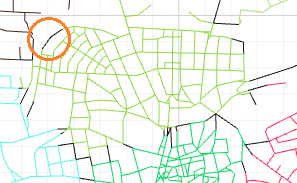
\includegraphics[width=\textwidth]{clusteranalysis_kmeans_problem.png}
    \end{mdframed}
    \caption{Problem of K-Means clustering
        \label{fig:KmeansProblem}}
\end{figure}

\subsubsection{Connected Cluster Results} \label{sec:K-Means_shortest_path}
To problem was then solved by using a \gls{APSP} algorithm like Dijkstra or Floyd-Warshall. In the following figure \ref{fig:Kmeansshortestp} every cluster is connected.

\begin{figure}
    \centering
    \begin{mdframed}[style=mdthight]
        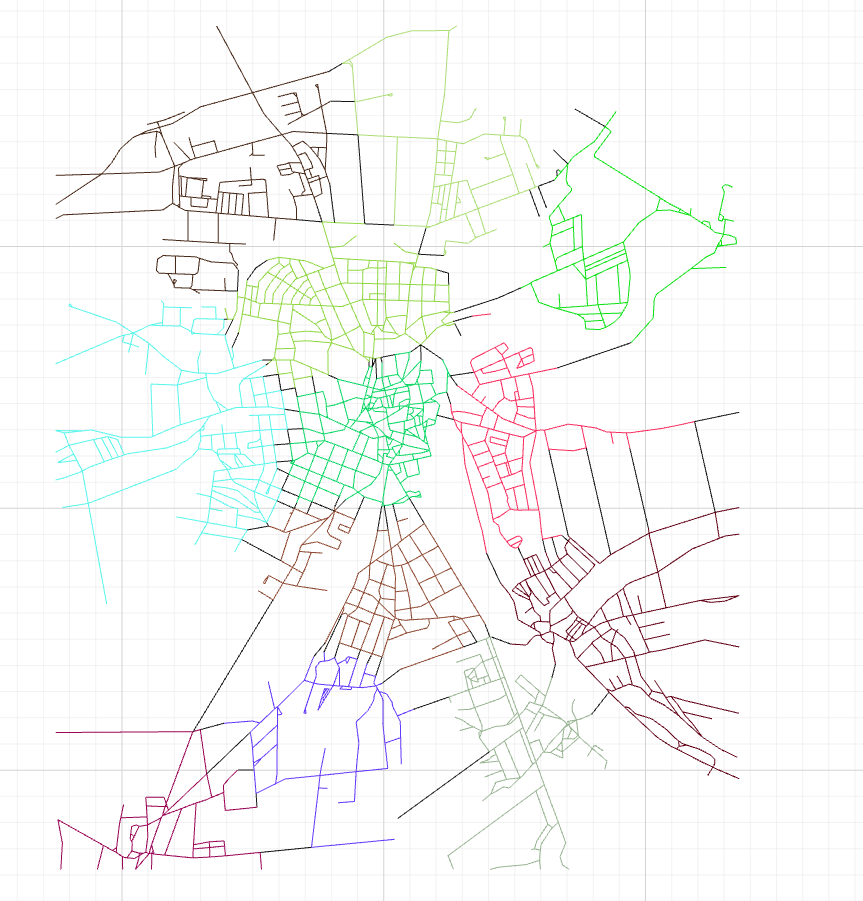
\includegraphics[width=\textwidth]{clusteranalysis_kmeans_result.png}
    \end{mdframed}
    \caption{K-Means cluster analysis of Weimar \label{fig:KmeansGenerated}}
\end{figure}

\begin{figure}
    \centering
    \begin{mdframed}[style=mdthight]
        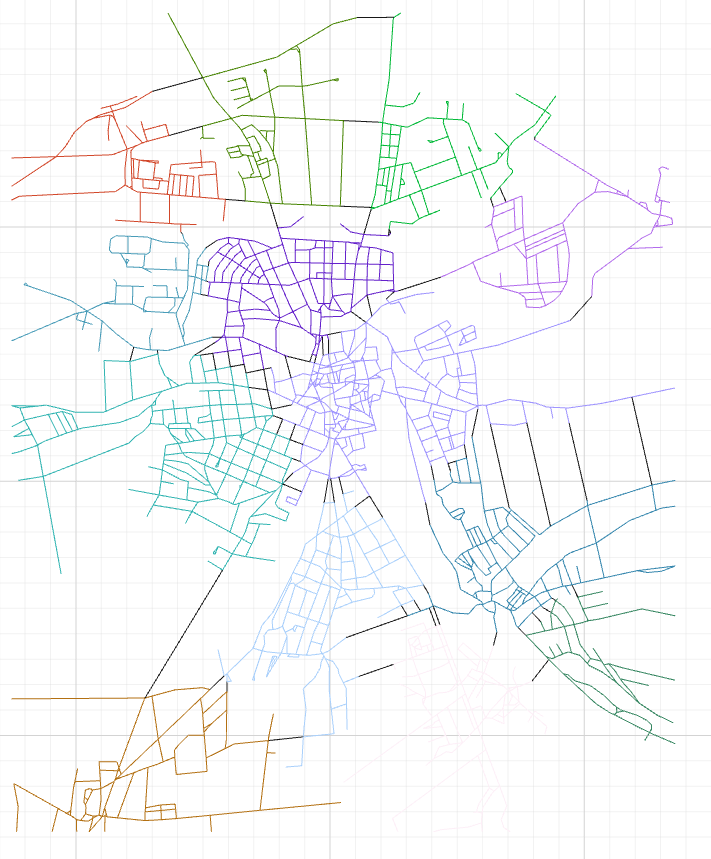
\includegraphics[width=\textwidth]{clusteranalysis_kmeansExt_result.png}
    \end{mdframed}
    \caption{K-Means clustering with shortest path\label{fig:Kmeansshortestp}}
\end{figure}
